\documentclass[../report/main.tex]{subfiles}
 
\begin{document}

\begin{enumerate}[a)]
	\item What are the lengths of the shortest paths from vertex $a$ to all other vertices?
    An image of the graph is below:

    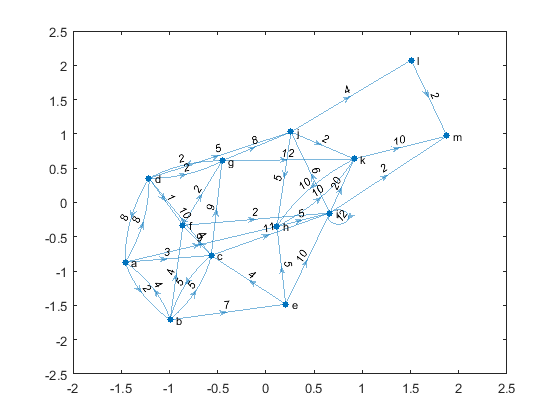
\includegraphics{../problem_three/problem3_digraph.png}

    The lengths of the shortest paths from a to the other vertices in the graph are listed below:
    \begin{itemize}
        \item a to b: 2
        \item a to c: 3
        \item a to d: 8
        \item a to e: 9
        \item a to f: 6
        \item a to g: 8
        \item a to h: 9
        \item a to i: 8
        \item a to j: 13
        \item a to k: 15
        \item a to l: 17
        \item a to m: 10
    \end{itemize}
	\item If a vertex $z$ is added to the graph for which there is no path from vertex $a$ to vertex $z$, what will be the result when you attempt to find the lengths of shortest paths as in part a).

The list will be the same except for the addition of the line 'a to z: Inf' which shows that you cannot access vertex z from a in the current graph because that is what was specified in the question.

	\item What are the lengths of the shortest paths from each vertex to vertex $m$? How can you solve this problem with just one linear program?

  \begin{itemize}
      \item a to m: 10
      \item b to m: 8
      \item c to m: 8
      \item d to m: 5
      \item e to m: 12
      \item f to m: 4
      \item g to m: 7
      \item h to m: 7
      \item i to m: 2
      \item j to m: 6
      \item k to m: 10
      \item l to m: 2
  \end{itemize}

	\item Suppose that all paths must pass through vertex $i$. How can you calculate the length of the shortest path from any vertex $x$ to vertex $y$ that pass through vertex $i$ (for all $x, y \in V$)? Calculate the lengths of these paths for the given graph. (Note: for some vertices $x$ and $y$, it may be impossible to pass through vertex $i$).
\end{enumerate}

\end{document}
